\documentclass[12pt,a4paper]{report}
\usepackage[utf8]{inputenc}
\usepackage[T1]{fontenc}
\usepackage[french]{babel}
\usepackage[margin=2.5cm]{geometry}
\usepackage{array}
\usepackage{longtable}
\usepackage{hyperref}
\usepackage{xcolor}
\usepackage{enumitem}
\usepackage{graphicx}
\usepackage{fancybox}
\usepackage{titlesec}
\usepackage{float}
\usepackage{caption}

\graphicspath{{images/}}

\hypersetup{
    colorlinks=true,
    linkcolor=blue,
    urlcolor=blue
}

\title{Description des Interfaces de l'Application\\SGRH Intelligent}
\author{MANSOUR Aymane \and FOUKOU Issa \and BADIA Salahedine}
\date{Année universitaire 2025--2026}

\begin{document}
\sloppy

\maketitle
\tableofcontents
\newpage

% =============================================================
\chapter{Introduction}
% =============================================================

Ce document présente les différentes interfaces graphiques de l'application \textbf{SGRH Intelligent} (Système de Gestion des Ressources Humaines avec Intelligence Artificielle). Chaque interface est décrite en détail : son rôle fonctionnel, les éléments visuels qui la composent, les actions disponibles pour l'utilisateur et les données affichées.

L'application est construite avec le framework React et utilise TailwindCSS pour le design. L'interface adopte une approche moderne, épurée et responsive, avec un menu latéral de navigation à gauche et un contenu principal à droite. Toutes les pages partagent un design cohérent avec des cartes (cards), des tableaux et des graphiques interactifs.

\section{Navigation générale}

L'interface comporte les éléments permanents suivants, visibles sur toutes les pages après connexion :

\begin{itemize}
    \item \textbf{Menu latéral (Sidebar)} : situé à gauche, il contient le logo \og SGRH Intelligent \fg{}, les liens de navigation vers chaque module, et en bas l'email de l'utilisateur connecté ainsi que le bouton de déconnexion.
    \item \textbf{Barre supérieure (Header)} : contient une barre de recherche globale, une icône de notifications et l'avatar de l'utilisateur avec son rôle.
    \item \textbf{Zone de contenu} : occupe le reste de l'écran et affiche la page active.
\end{itemize}

Les modules accessibles dans le menu dépendent du rôle de l'utilisateur :
\begin{itemize}
    \item \textbf{ADMIN} : Tableau de bord, Employés, Congés, Présences, Paie, Documents, Analyse IA, Utilisateurs
    \item \textbf{RH} : Tableau de bord, Employés, Congés, Présences, Paie, Documents, Analyse IA
    \item \textbf{EMPLOYE} : Tableau de bord, Congés, Présences, Documents
\end{itemize}

% =============================================================
\chapter{Page de connexion (Login)}
% =============================================================

\section{Capture d'écran}

\begin{figure}[H]
\centering

\includegraphics[width=\textwidth]{page_lgine.png}
\caption{Interface de connexion de l'application SGRH Intelligent}
\label{fig:login}
\end{figure}

\section{Accès}
\begin{itemize}
    \item \textbf{URL} : \texttt{http://localhost:3000/login}
    \item \textbf{Fichier source} : \texttt{frontend/src/pages/LoginPage.jsx}
    \item \textbf{Rôles concernés} : Tous les utilisateurs non connectés
\end{itemize}

\section{Description visuelle}

La page de connexion est divisée en deux parties :

\subsection{Panneau gauche (Branding)}

Ce panneau occupe la moitié gauche de l'écran (visible uniquement sur les grands écrans). Il présente :
\begin{itemize}
    \item Le logo de l'application avec l'icône \og Brain \fg{} (cerveau) symbolisant l'intelligence artificielle
    \item Le titre \textbf{SGRH Intelligent}
    \item Une description : \og Système de Gestion des Ressources Humaines avec Intelligence Artificielle et Analyse OCR de Documents \fg{}
    \item Trois cartes présentant les fonctionnalités principales :
    \begin{itemize}
        \item \textbf{IA} — Détection anomalies
        \item \textbf{OCR} — Analyse documents
        \item \textbf{RH} — Gestion complète
    \end{itemize}
\end{itemize}

Le fond est un dégradé bleu foncé avec des effets de transparence (\textit{backdrop-blur}) qui donnent un aspect moderne et professionnel.

\subsection{Panneau droit (Formulaire)}

Ce panneau contient le formulaire de connexion avec les éléments suivants :
\begin{itemize}
    \item \textbf{Titre} : \og Connexion \fg{}
    \item \textbf{Sous-titre} : \og Accédez à votre espace de gestion RH \fg{}
    \item \textbf{Champ Email} : champ texte avec une icône d'enveloppe, placeholder \og votre@email.ma \fg{}
    \item \textbf{Champ Mot de passe} : champ sécurisé avec une icône de cadenas et un bouton \og œil \fg{} pour afficher/masquer le mot de passe
    \item \textbf{Bouton Se connecter} : bouton bleu occupant toute la largeur, avec animation de chargement lors de l'envoi
    \item \textbf{Mode démonstration} : trois boutons secondaires (Admin, RH, Employé) permettant de se connecter sans backend pour tester l'interface
\end{itemize}

\section{Comportement fonctionnel}

\begin{enumerate}
    \item L'utilisateur saisit son email et son mot de passe
    \item Il clique sur \og Se connecter \fg{}
    \item Le frontend envoie une requête POST à \texttt{/api/auth/login}
    \item En cas de succès : le token JWT est stocké dans le \texttt{localStorage} et l'utilisateur est redirigé vers le tableau de bord
    \item En cas d'erreur : un message \og Identifiants incorrects \fg{} s'affiche sous forme de notification toast
\end{enumerate}

\section{Identifiants par défaut}

\begin{longtable}{|p{5cm}|p{4cm}|p{3cm}|}
\hline
\textbf{Email} & \textbf{Mot de passe} & \textbf{Rôle} \\
\hline
\texttt{admin@sgrh.ma} & \texttt{password123} & ADMIN \\
\hline
\texttt{rh@sgrh.ma} & \texttt{password123} & RH \\
\hline
\texttt{ahmed.benali@sgrh.ma} & \texttt{password123} & EMPLOYE \\
\hline
\end{longtable}

% =============================================================
\chapter{Tableau de bord (Dashboard)}
% =============================================================

\section{Capture d'écran}

\begin{figure}[H]
\centering
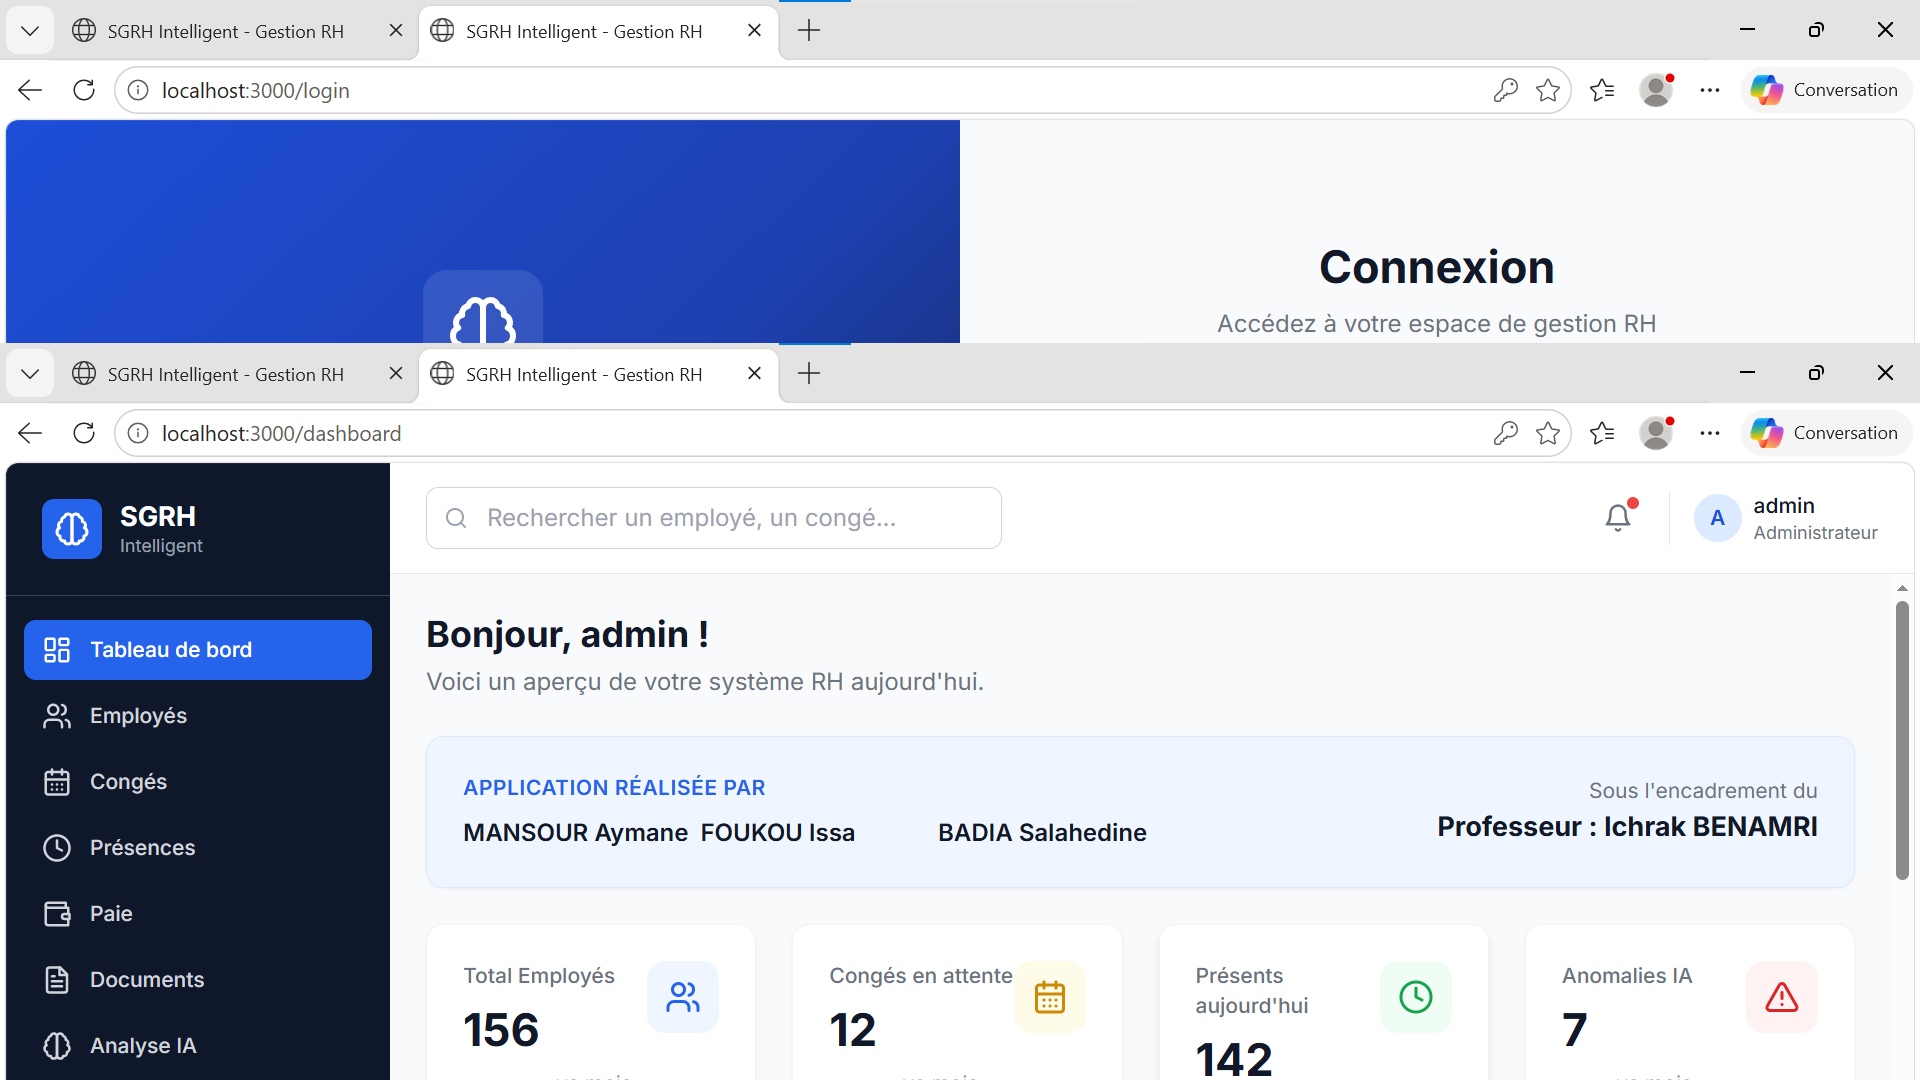
\includegraphics[width=\textwidth]{Tableau_Bord.png}
\caption{Tableau de bord -- vue d'ensemble avec statistiques et graphiques}
\label{fig:dashboard}
\end{figure}

\section{Accès}
\begin{itemize}
    \item \textbf{URL} : \texttt{http://localhost:3000/dashboard}
    \item \textbf{Fichier source} : \texttt{frontend/src/pages/DashboardPage.jsx}
    \item \textbf{Rôles concernés} : ADMIN, RH, EMPLOYE
\end{itemize}

\section{Description visuelle}

Le tableau de bord est la page d'accueil après connexion. Il offre une vue synthétique de l'état du système RH.

\subsection{En-tête de bienvenue}

\begin{itemize}
    \item Message personnalisé : \og Bonjour, [nom] ! \fg{}
    \item Sous-titre : \og Voici un aperçu de votre système RH aujourd'hui. \fg{}
\end{itemize}

\subsection{Bandeau projet}

Un encadré indique les réalisateurs du projet :
\begin{itemize}
    \item \textbf{Application réalisée par} : MANSOUR Aymane, FOUKOU Issa, BADIA Salahedine
    \item \textbf{Sous l'encadrement du Professeur} : Ichrak BENAMRI
\end{itemize}

\subsection{Cartes statistiques}

Quatre cartes alignées horizontalement affichent les indicateurs clés :
\begin{enumerate}
    \item \textbf{Total Employés} : nombre total d'employés enregistrés (ex: 156), avec variation mensuelle (+3.2\%)
    \item \textbf{Congés en attente} : nombre de demandes de congé non traitées (ex: 12), avec variation (-8\%)
    \item \textbf{Présents aujourd'hui} : nombre d'employés pointés présents (ex: 142), avec variation (+1.5\%)
    \item \textbf{Anomalies IA} : nombre d'anomalies comportementales détectées (ex: 7), avec variation (-2)
\end{enumerate}

Chaque carte possède une icône colorée distinctive (vert pour employés, orange pour congés, bleu pour présences, rouge pour anomalies).

\subsection{Graphiques}

\begin{itemize}
    \item \textbf{Congés par mois} : graphique en barres montrant l'évolution mensuelle des demandes de congé avec un lien \og Voir tout \fg{}
    \item \textbf{Par département} : graphique circulaire (donut) montrant la répartition des employés par département
\end{itemize}

\section{Comportement fonctionnel}

Les données affichées sont récupérées depuis l'endpoint \texttt{/api/dashboard/stats} du backend. Les statistiques sont calculées en temps réel à partir de la base de données. Les variations sont calculées par rapport au mois précédent.

% =============================================================
\chapter{Gestion des Employés}
% =============================================================

\section{Capture d'écran}

\begin{figure}[H]
\centering
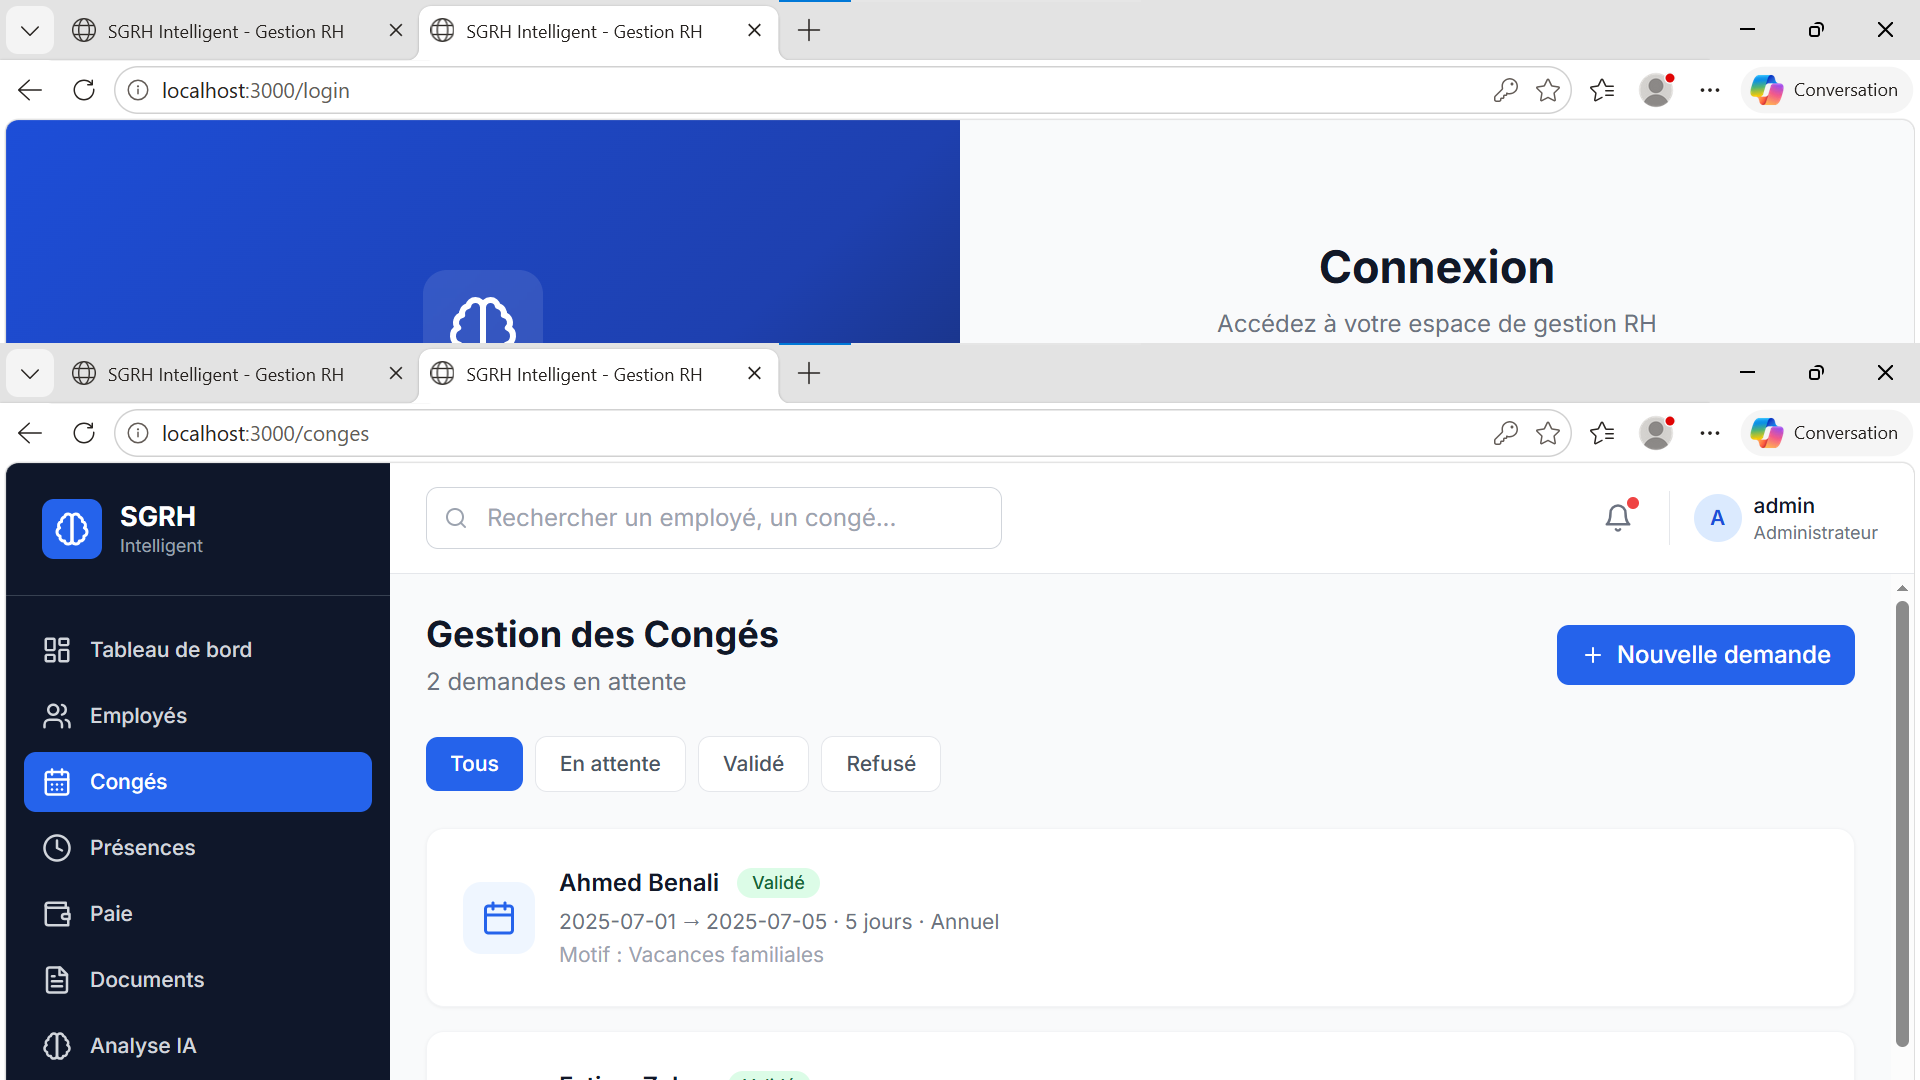
\includegraphics[width=\textwidth]{Gestion_Employes.png}
\caption{Interface de gestion des employés avec tableau et actions CRUD}
\label{fig:employes}
\end{figure}

\section{Accès}
\begin{itemize}
    \item \textbf{URL} : \texttt{http://localhost:3000/employes}
    \item \textbf{Fichier source} : \texttt{frontend/src/pages/EmployesPage.jsx}
    \item \textbf{Rôles concernés} : ADMIN, RH
\end{itemize}

\section{Description visuelle}

\subsection{En-tête}

\begin{itemize}
    \item Titre : \og Gestion des Employés \fg{}
    \item Sous-titre : \og Gérez les informations de vos collaborateurs \fg{}
    \item Bouton \textbf{+ Ajouter} : ouvre un formulaire modal de création d'employé
    \item Barre de recherche avec icône loupe : permet de filtrer les employés par nom, prénom, matricule ou département
\end{itemize}

\subsection{Tableau des employés}

Un tableau affiche la liste de tous les employés avec les colonnes suivantes :
\begin{itemize}
    \item \textbf{Matricule} : identifiant unique (ex: EMP-001)
    \item \textbf{Nom complet} : nom et prénom de l'employé
    \item \textbf{Poste} : intitulé du poste occupé (ex: Développeur Full-Stack)
    \item \textbf{Département} : département de rattachement (ex: IT, Finance, Marketing)
    \item \textbf{Salaire} : salaire brut mensuel en MAD
    \item \textbf{Solde congé} : nombre de jours de congé restants
    \item \textbf{Statut} : badge coloré indiquant si l'employé est actif (vert) ou inactif (rouge)
    \item \textbf{Actions} : trois icônes — voir (œil), modifier (crayon), supprimer (corbeille)
\end{itemize}

\subsection{Modal de création/modification}

Lorsqu'on clique sur \og Ajouter \fg{} ou \og Modifier \fg{}, un formulaire modal s'affiche avec les champs :
\begin{itemize}
    \item Matricule, Nom, Prénom, Poste, Département, Salaire, Email, Solde congé, Statut actif
\end{itemize}

\section{Comportement fonctionnel}

\begin{itemize}
    \item \textbf{Créer} : envoie une requête POST à \texttt{/api/employes}
    \item \textbf{Modifier} : envoie une requête PUT à \texttt{/api/employes/\{id\}}
    \item \textbf{Supprimer} : confirmation, puis requête DELETE à \texttt{/api/employes/\{id\}}
    \item \textbf{Recherche} : filtrage côté client en temps réel
\end{itemize}

% =============================================================
\chapter{Gestion des Congés}
% =============================================================

\section{Capture d'écran}

\begin{figure}[H]
\centering
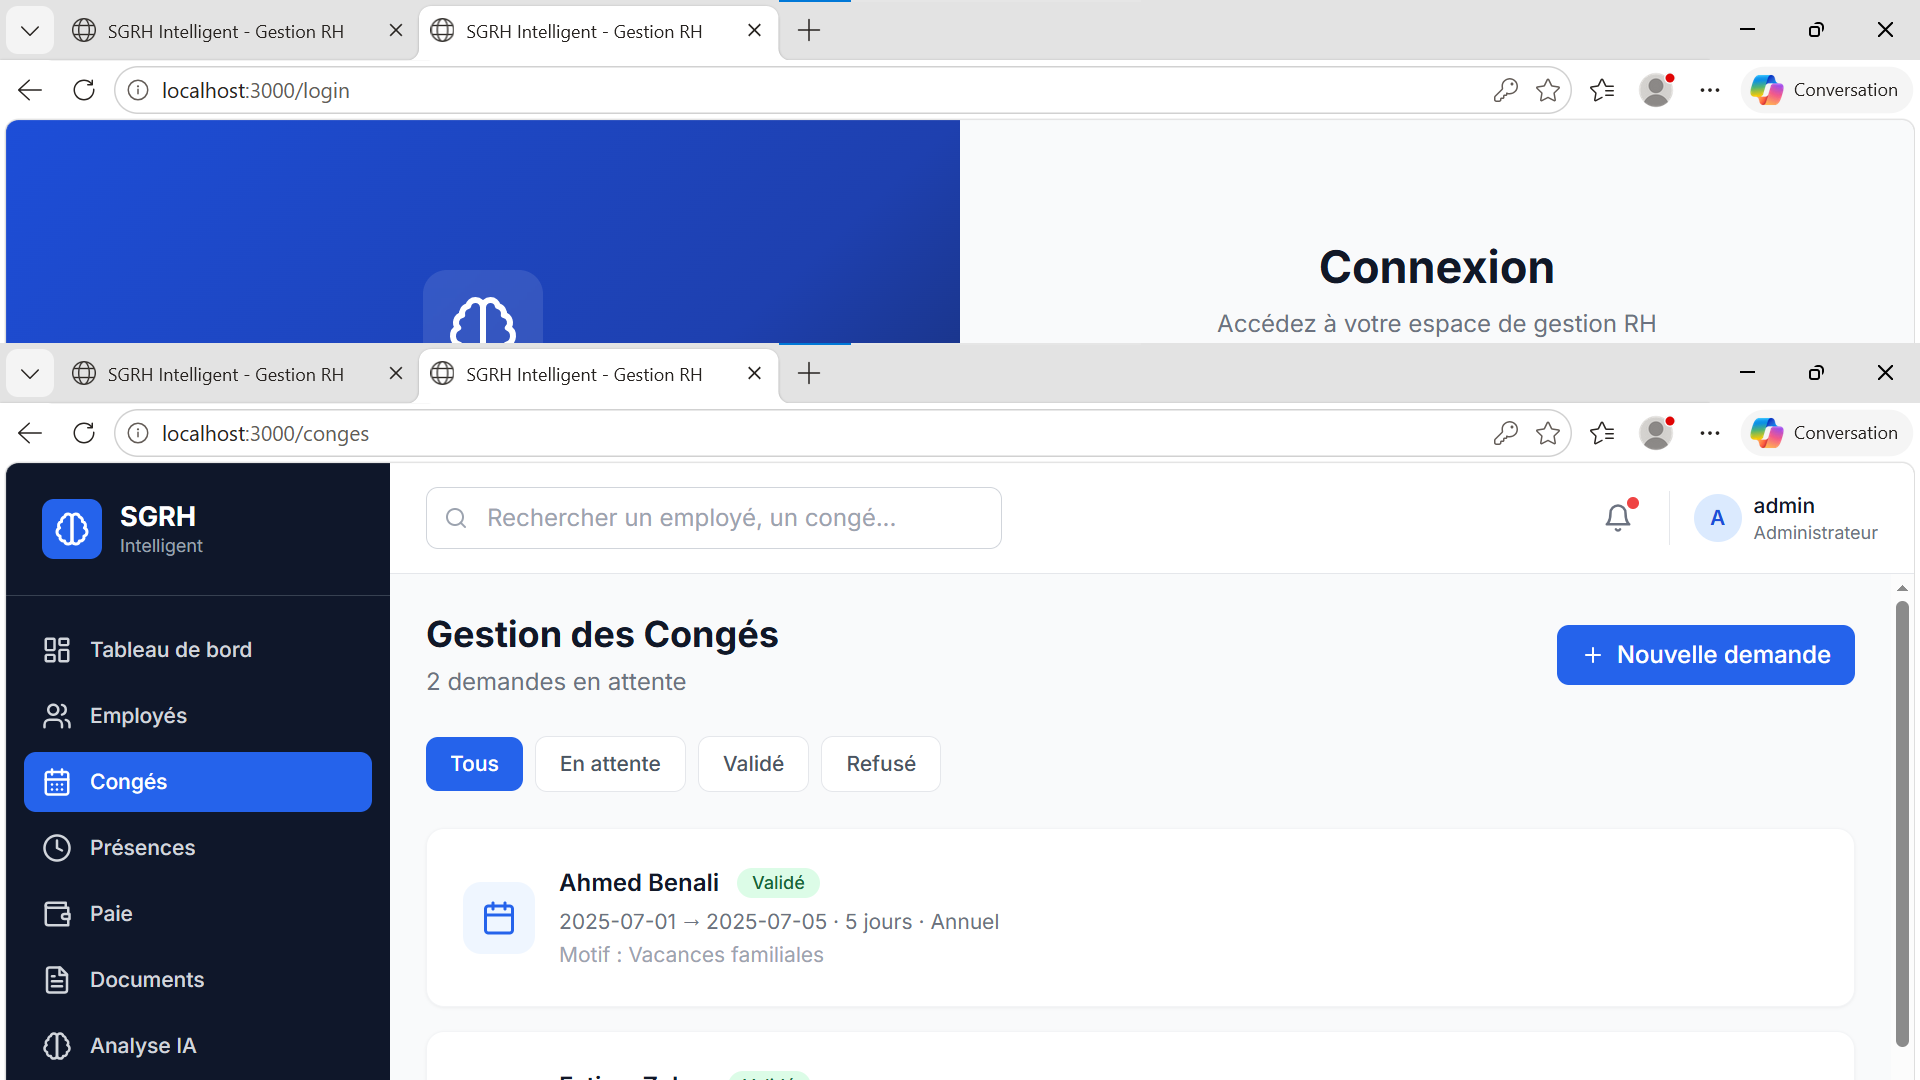
\includegraphics[width=\textwidth]{Gestion_Conges.png}
\caption{Interface de gestion des congés avec filtres et validation}
\label{fig:conges}
\end{figure}

\section{Accès}
\begin{itemize}
    \item \textbf{URL} : \texttt{http://localhost:3000/conges}
    \item \textbf{Fichier source} : \texttt{frontend/src/pages/CongesPage.jsx}
    \item \textbf{Rôles concernés} : ADMIN, RH, EMPLOYE
\end{itemize}

\section{Description visuelle}

\subsection{En-tête}

\begin{itemize}
    \item Titre : \og Gestion des Congés \fg{}
    \item Sous-titre : \og Demandes et validation des congés \fg{}
    \item Bouton \textbf{+ Nouvelle demande} : ouvre un formulaire de soumission de congé
    \item Filtres de statut : boutons \og Tous \fg{}, \og En attente \fg{}, \og Validés \fg{}, \og Refusés \fg{} pour filtrer la liste
\end{itemize}

\subsection{Tableau des congés}

Le tableau affiche toutes les demandes de congé avec les colonnes :
\begin{itemize}
    \item \textbf{Employé} : nom de l'employé demandeur
    \item \textbf{Date début} : date de début du congé
    \item \textbf{Date fin} : date de fin du congé
    \item \textbf{Durée} : nombre de jours
    \item \textbf{Type} : type de congé (Annuel, Maladie, Sans solde)
    \item \textbf{Motif} : raison invoquée
    \item \textbf{Statut} : badge coloré — jaune (En attente), vert (Validé), rouge (Refusé)
    \item \textbf{Actions} (RH/Admin uniquement) : boutons Valider (coche verte) et Refuser (croix rouge)
\end{itemize}

\subsection{Modal de demande de congé}

Le formulaire de demande contient :
\begin{itemize}
    \item Date de début, Date de fin, Type de congé (liste déroulante), Motif (zone de texte)
\end{itemize}

\section{Comportement fonctionnel}

\begin{itemize}
    \item \textbf{Soumettre une demande} : POST à \texttt{/api/conges}
    \item \textbf{Valider} (RH/Admin) : PUT à \texttt{/api/conges/\{id\}/valider} — décrémente automatiquement le solde de congé de l'employé
    \item \textbf{Refuser} (RH/Admin) : PUT à \texttt{/api/conges/\{id\}/refuser}
    \item Un employé ne peut voir et soumettre que ses propres demandes. Un RH ou Admin voit toutes les demandes.
\end{itemize}

% =============================================================
\chapter{Gestion des Présences}
% =============================================================

\section{Capture d'écran}

\begin{figure}[H]
\centering
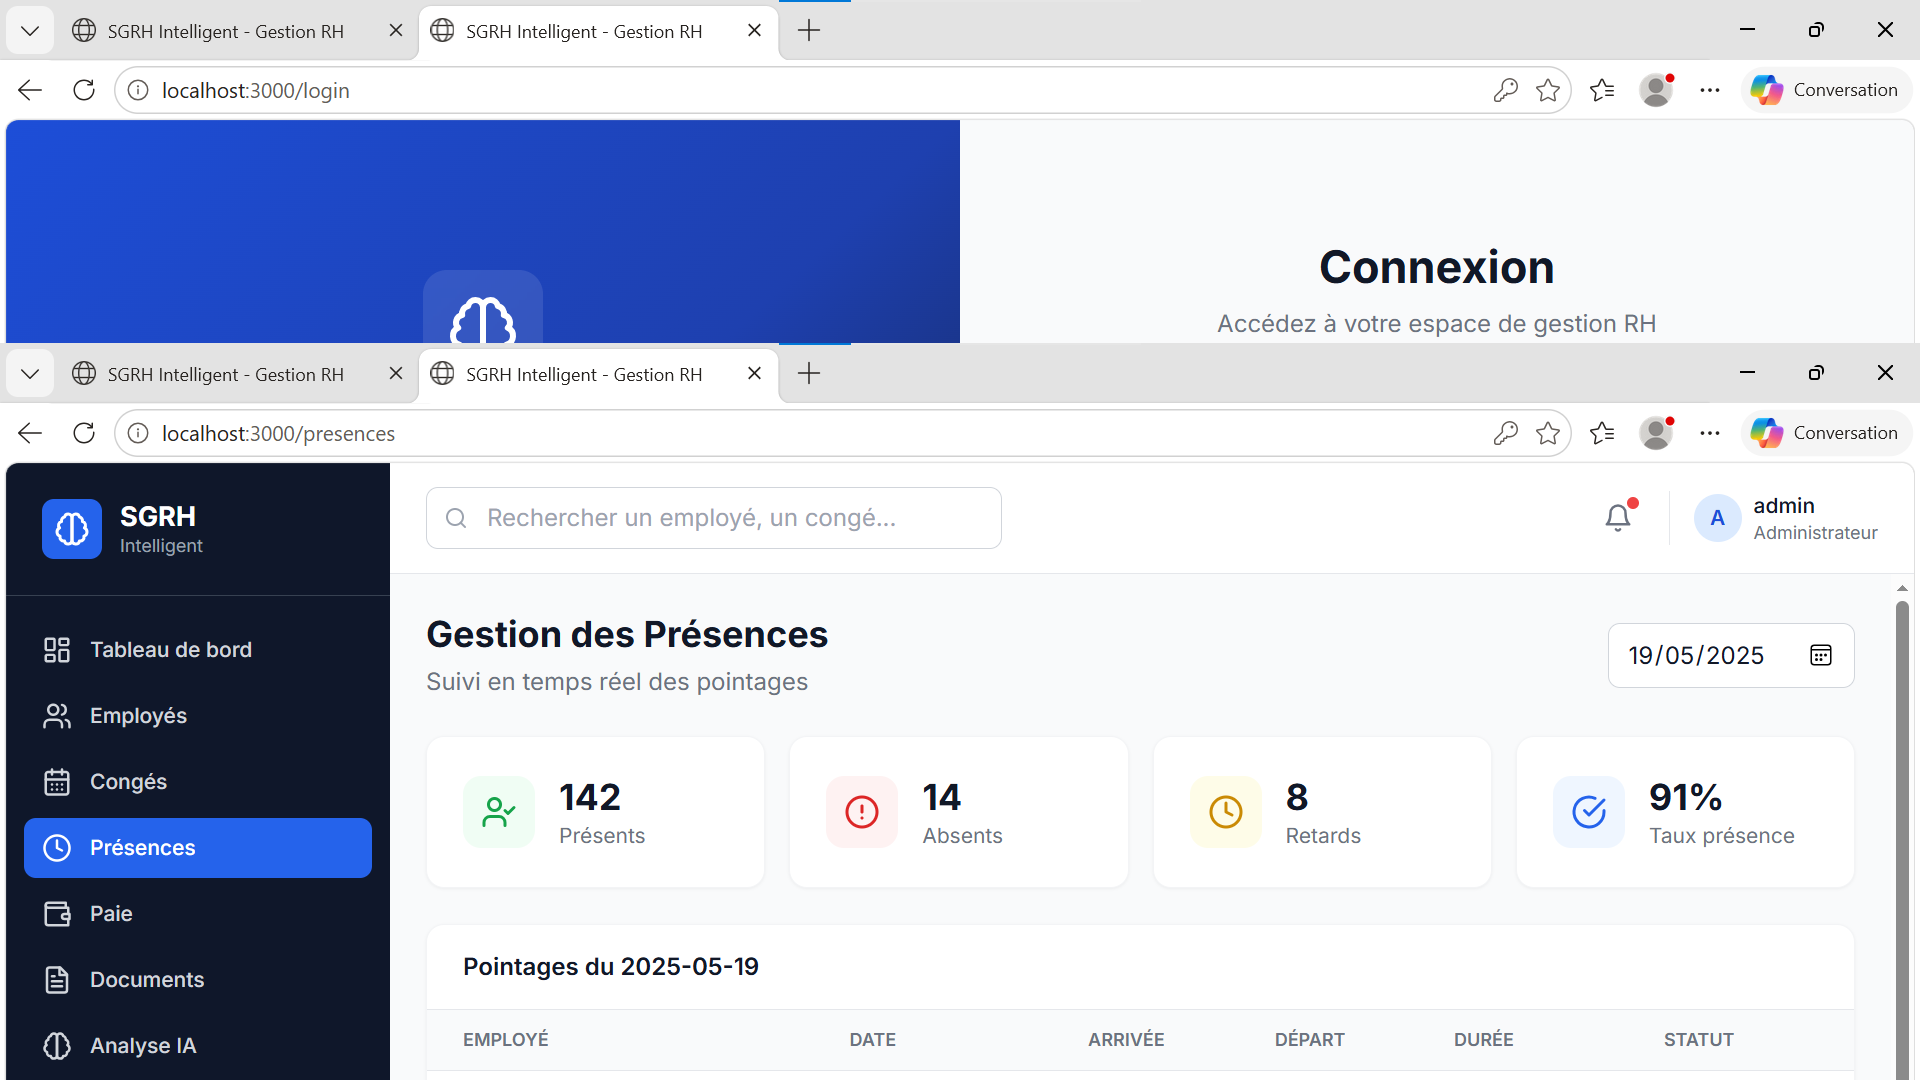
\includegraphics[width=\textwidth]{Gestion_Presences.png}
\caption{Interface de suivi des présences et pointages}
\label{fig:presences}
\end{figure}

\section{Accès}
\begin{itemize}
    \item \textbf{URL} : \texttt{http://localhost:3000/presences}
    \item \textbf{Fichier source} : \texttt{frontend/src/pages/PresencesPage.jsx}
    \item \textbf{Rôles concernés} : ADMIN, RH, EMPLOYE
\end{itemize}

\section{Description visuelle}

\subsection{En-tête}

\begin{itemize}
    \item Titre : \og Gestion des Présences \fg{}
    \item Sous-titre : \og Suivi en temps réel des pointages \fg{}
    \item Sélecteur de date : champ permettant de choisir la journée à consulter
\end{itemize}

\subsection{Cartes statistiques}

Quatre cartes affichent les indicateurs de la journée sélectionnée :
\begin{enumerate}
    \item \textbf{Présents} : nombre d'employés ayant pointé (icône verte, ex: 142)
    \item \textbf{Absents} : nombre d'employés n'ayant pas pointé (icône rouge, ex: 14)
    \item \textbf{Retards} : nombre d'arrivées après l'heure réglementaire (icône jaune, ex: 8)
    \item \textbf{Taux de présence} : pourcentage de présence global (icône bleue, ex: 91\%)
\end{enumerate}

\subsection{Tableau des pointages}

Le tableau affiche les enregistrements de présence avec :
\begin{itemize}
    \item \textbf{Employé} : nom complet
    \item \textbf{Date} : date du pointage
    \item \textbf{Heure d'arrivée} : heure d'entrée (ex: 08:30)
    \item \textbf{Heure de départ} : heure de sortie (ex: 17:00)
    \item \textbf{Durée} : temps de travail effectif calculé automatiquement
    \item \textbf{Ponctualité} : badge indiquant \og À l'heure \fg{} (vert) ou \og En retard \fg{} (rouge)
\end{itemize}

\section{Comportement fonctionnel}

\begin{itemize}
    \item Les données proviennent de l'endpoint \texttt{/api/presences}
    \item Le filtrage par date envoie une requête à \texttt{/api/presences?date=YYYY-MM-DD}
    \item Un employé est considéré en retard si son heure d'arrivée dépasse 08:15
    \item Le pointage peut être enregistré via POST à \texttt{/api/presences}
\end{itemize}

% =============================================================
\chapter{Gestion de la Paie}
% =============================================================

\section{Capture d'écran}

\begin{figure}[H]
\centering
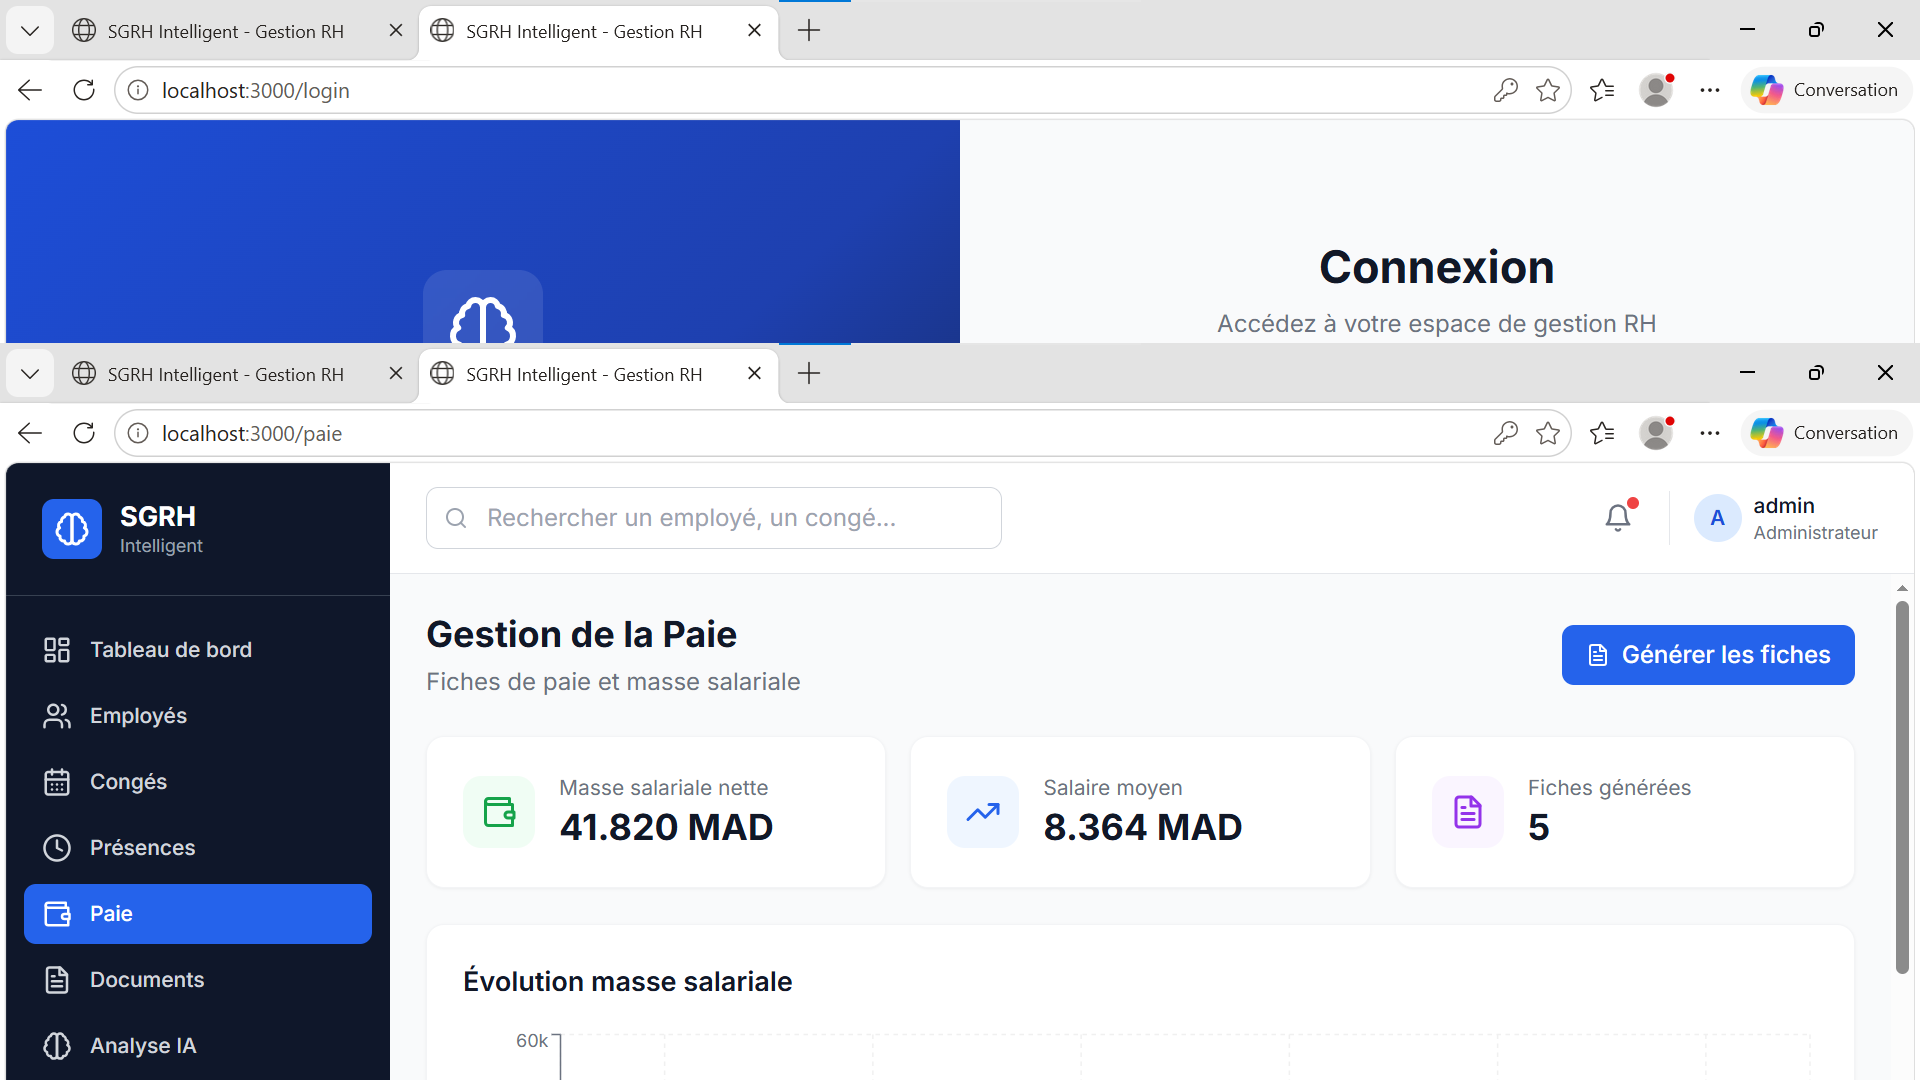
\includegraphics[width=\textwidth]{Gestion_Paie.png}
\caption{Interface de gestion de la paie avec graphique d'évolution}
\label{fig:paie}
\end{figure}

\section{Accès}
\begin{itemize}
    \item \textbf{URL} : \texttt{http://localhost:3000/paie}
    \item \textbf{Fichier source} : \texttt{frontend/src/pages/PaiePage.jsx}
    \item \textbf{Rôles concernés} : ADMIN, RH
\end{itemize}

\section{Description visuelle}

\subsection{En-tête}

\begin{itemize}
    \item Titre : \og Gestion de la Paie \fg{}
    \item Sous-titre : \og Fiches de paie et masse salariale \fg{}
    \item Bouton \textbf{Générer les fiches} : lance la génération automatique des fiches de paie pour le mois en cours
\end{itemize}

\subsection{Cartes statistiques}

Trois cartes affichent les indicateurs financiers :
\begin{enumerate}
    \item \textbf{Masse salariale nette} : somme totale des salaires nets du mois (icône verte, ex: 41\,820 MAD)
    \item \textbf{Salaire moyen} : moyenne des salaires nets (icône bleue, ex: 8\,364 MAD)
    \item \textbf{Fiches générées} : nombre de fiches produites (icône violette, ex: 5)
\end{enumerate}

\subsection{Graphique d'évolution}

Un graphique en barres verticales montre l'évolution de la masse salariale sur les 6 derniers mois (janvier à juin). L'axe Y affiche les montants en milliers de MAD, chaque barre est colorée en violet avec des coins arrondis.

\subsection{Tableau des fiches de paie}

Le tableau détaille les fiches individuelles avec :
\begin{itemize}
    \item \textbf{Employé} : nom complet
    \item \textbf{Période} : mois et année (ex: Mai 2025)
    \item \textbf{Salaire Brut} : montant brut en MAD
    \item \textbf{Salaire Net} : montant net en MAD (après déductions)
    \item \textbf{Actions} : lien \og Télécharger \fg{} pour exporter la fiche en PDF
\end{itemize}

Un bouton \textbf{Exporter PDF} en haut du tableau permet de télécharger l'ensemble des fiches.

\section{Comportement fonctionnel}

\begin{itemize}
    \item Les fiches proviennent de \texttt{/api/fiches-paie}
    \item La génération automatique appelle \texttt{/api/fiches-paie/generer}
    \item Le salaire net est calculé à partir du salaire brut avec les déductions légales (environ 18\% de retenues)
\end{itemize}

% =============================================================
\chapter{Gestion des Documents}
% =============================================================

\section{Capture d'écran}

\begin{figure}[H]
\centering
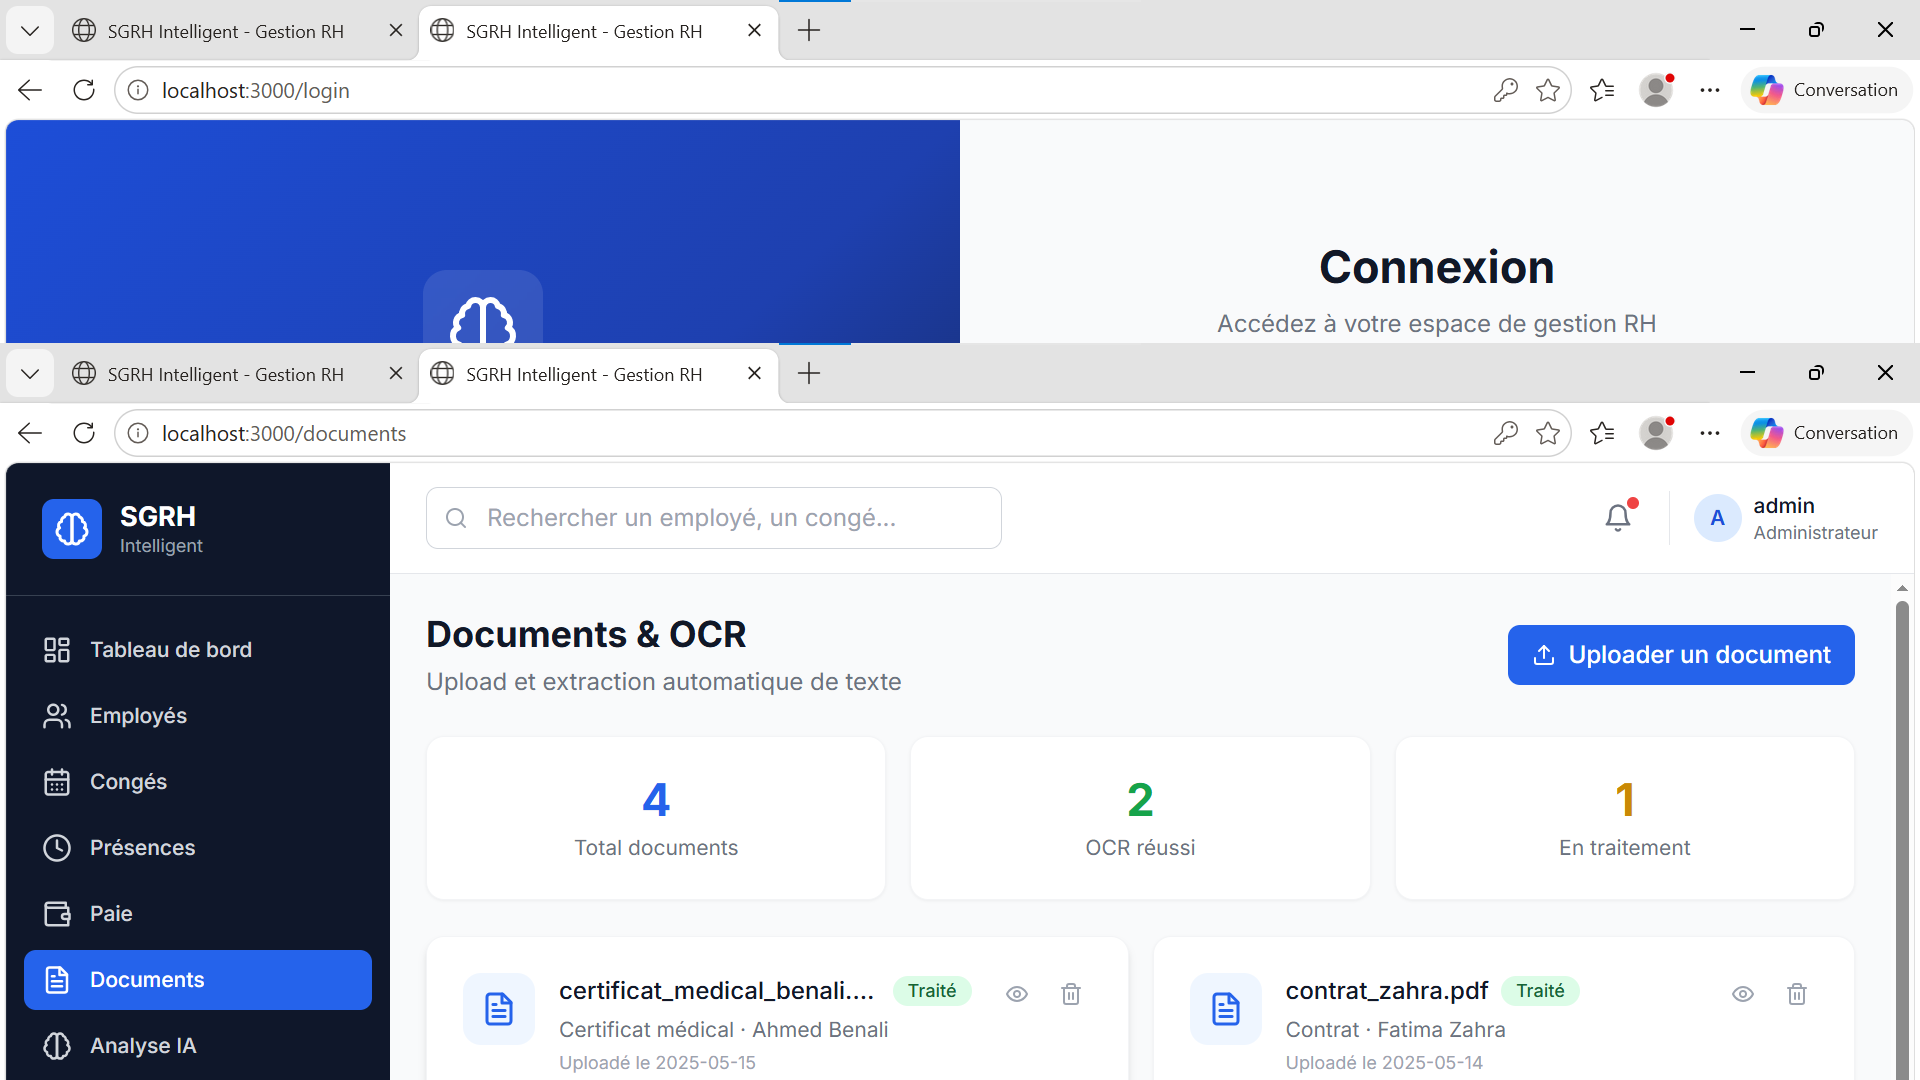
\includegraphics[width=\textwidth]{Documents_OCR.png}
\caption{Interface de gestion des documents avec traitement OCR}
\label{fig:documents}
\end{figure}

\section{Accès}
\begin{itemize}
    \item \textbf{URL} : \texttt{http://localhost:3000/documents}
    \item \textbf{Fichier source} : \texttt{frontend/src/pages/DocumentsPage.jsx}
    \item \textbf{Rôles concernés} : ADMIN, RH, EMPLOYE
\end{itemize}

\section{Description visuelle}

\subsection{En-tête}

\begin{itemize}
    \item Titre : \og Documents \& OCR \fg{}
    \item Sous-titre : \og Upload et analyse intelligente de documents \fg{}
    \item Bouton \textbf{+ Upload} : ouvre une zone de dépôt de fichier pour téléverser un nouveau document
\end{itemize}

\subsection{Zone d'upload}

Lorsque le bouton Upload est cliqué, une zone de dépôt (drag \& drop) s'affiche avec :
\begin{itemize}
    \item Une icône de téléversement
    \item Le texte \og Glissez un fichier ou cliquez pour sélectionner \fg{}
    \item Les formats acceptés : PDF, JPG, PNG
    \item Taille maximale : 10 Mo
\end{itemize}

\subsection{Tableau des documents}

Le tableau liste les documents déjà téléversés :
\begin{itemize}
    \item \textbf{Nom du fichier} : nom original du document
    \item \textbf{Type} : format du fichier (PDF, Image)
    \item \textbf{Date d'upload} : date de téléversement
    \item \textbf{Statut OCR} : badge indiquant l'état du traitement — \og Traité \fg{} (vert), \og En cours \fg{} (jaune), \og En attente \fg{} (gris)
    \item \textbf{Actions} : icônes pour voir le détail (œil) et supprimer (corbeille)
\end{itemize}

\subsection{Vue détaillée d'un document}

En cliquant sur l'icône \og voir \fg{}, un panneau affiche :
\begin{itemize}
    \item Les métadonnées du document (nom, taille, date)
    \item Le texte extrait par l'OCR Tesseract
\end{itemize}

\section{Comportement fonctionnel}

\begin{itemize}
    \item \textbf{Upload} : envoie le fichier en multipart à \texttt{/api/documents/upload}
    \item Le backend sauvegarde le fichier sur le disque et lance le traitement OCR via Tesseract
    \item Le texte extrait est stocké dans la base de données associé au document
    \item \textbf{Suppression} : DELETE à \texttt{/api/documents/\{id\}}
\end{itemize}

% =============================================================
\chapter{Analyse IA}
% =============================================================

\section{Capture d'écran}

\begin{figure}[H]
\centering
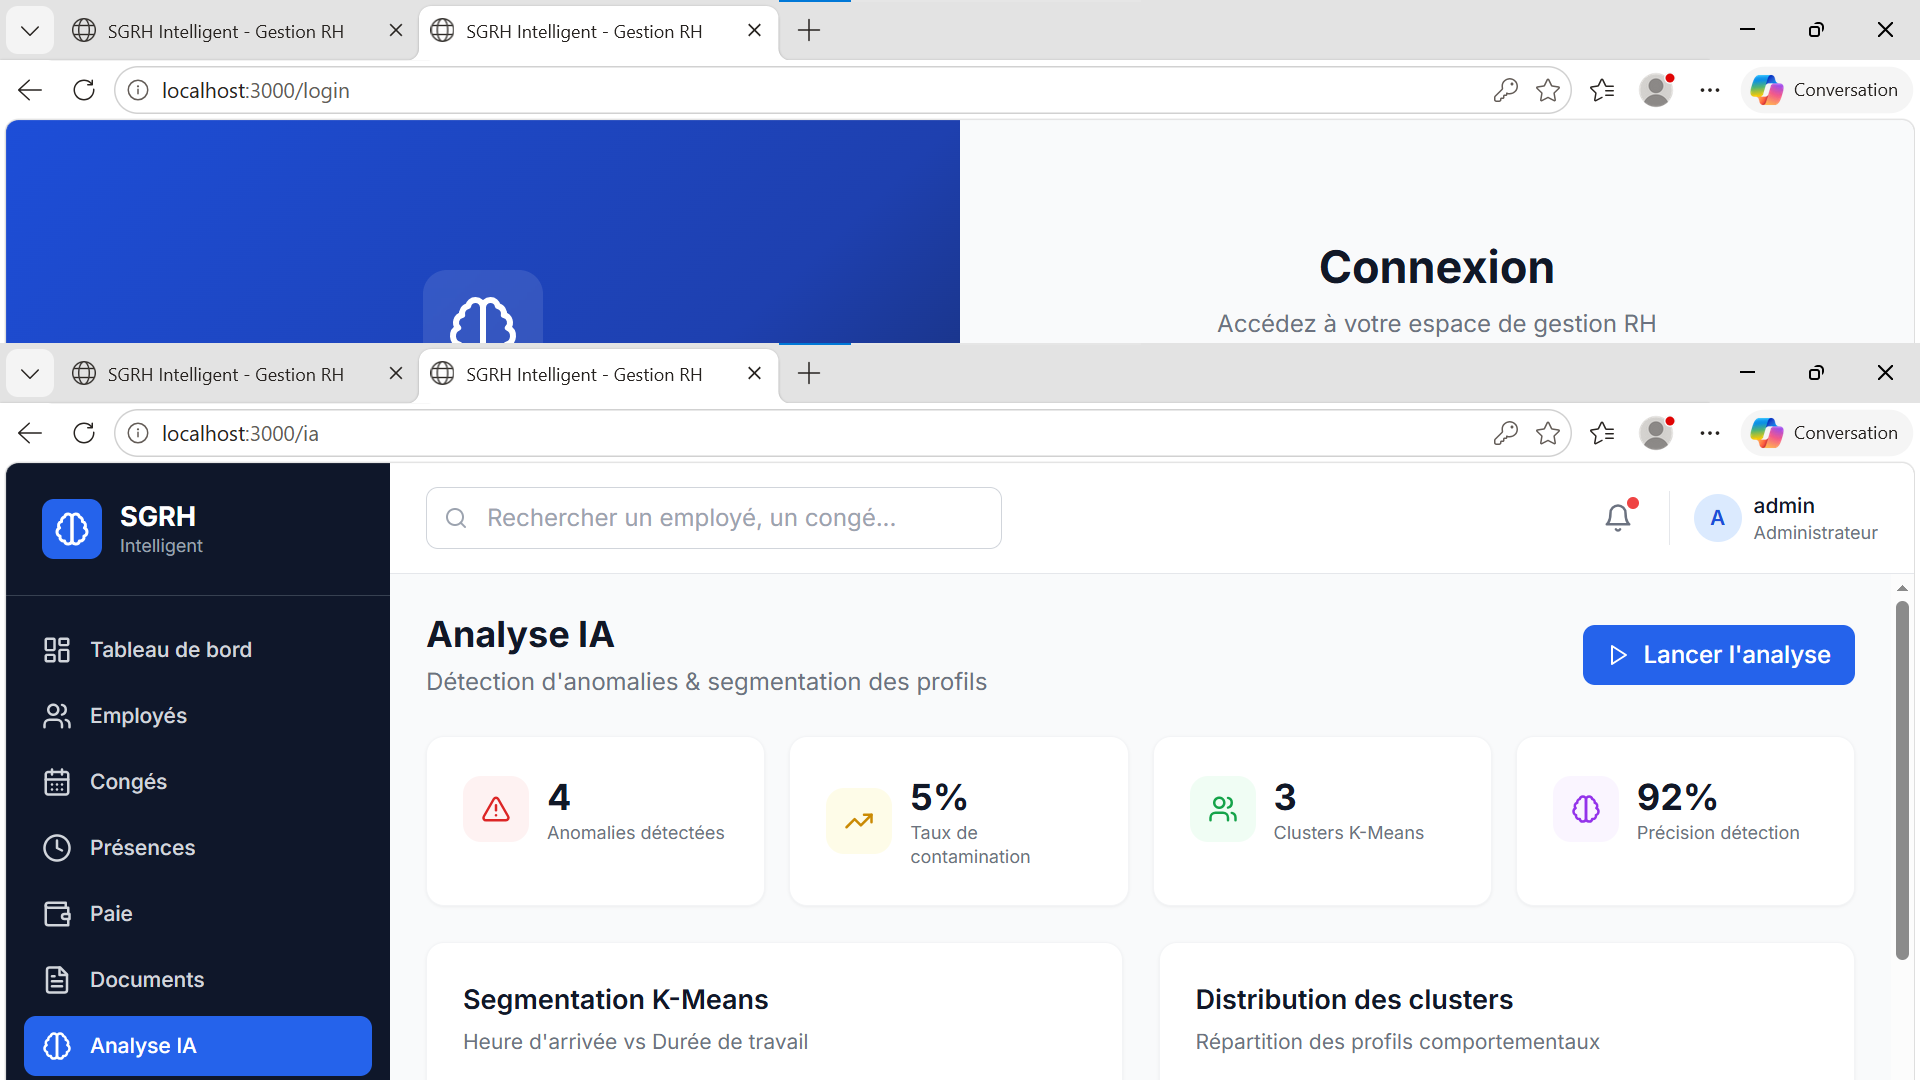
\includegraphics[width=\textwidth]{Analyse_IA.png}
\caption{Interface d'analyse IA -- détection d'anomalies et segmentation K-Means}
\label{fig:ia}
\end{figure}

\section{Accès}
\begin{itemize}
    \item \textbf{URL} : \texttt{http://localhost:3000/analyse-ia}
    \item \textbf{Fichier source} : \texttt{frontend/src/pages/IAPage.jsx}
    \item \textbf{Rôles concernés} : ADMIN, RH
\end{itemize}

\section{Description visuelle}

\subsection{En-tête}

\begin{itemize}
    \item Titre : \og Analyse IA \fg{}
    \item Sous-titre : \og Détection d'anomalies \& segmentation des profils \fg{}
    \item Bouton \textbf{Lancer l'analyse} : déclenche l'exécution des algorithmes IA (avec animation de chargement)
\end{itemize}

\subsection{Cartes statistiques IA}

Quatre cartes présentent les résultats synthétiques :
\begin{enumerate}
    \item \textbf{Anomalies détectées} : nombre total d'anomalies (icône rouge, ex: 4)
    \item \textbf{Taux de contamination} : pourcentage d'employés présentant un comportement anormal (icône jaune, ex: 5\%)
    \item \textbf{Clusters K-Means} : nombre de groupes identifiés par la segmentation (icône verte, ex: 3)
    \item \textbf{Précision détection} : score de précision du modèle Isolation Forest (icône violette, ex: 92\%)
\end{enumerate}

\subsection{Graphiques d'analyse}

Deux graphiques côte à côte :

\begin{itemize}
    \item \textbf{Segmentation K-Means (Scatter Plot)} : un nuage de points colorés représentant les employés selon deux axes — \og Heure d'arrivée \fg{} (X) et \og Durée de travail \fg{} (Y). Chaque couleur correspond à un cluster :
    \begin{itemize}
        \item Vert = Normal (employés ponctuels avec durée de travail complète)
        \item Jaune = Retardataire (arrivées tardives)
        \item Rouge = Absent (peu de temps de travail)
    \end{itemize}
    \item \textbf{Distribution des clusters (Pie Chart)} : un graphique circulaire en anneau (donut) montrant la proportion de chaque cluster — Normal (85\%), Retardataire (10\%), Absent (5\%)
\end{itemize}

\subsection{Tableau des anomalies}

Un tableau détaillé liste les anomalies détectées par l'algorithme Isolation Forest :
\begin{itemize}
    \item \textbf{Employé} : nom de l'employé concerné
    \item \textbf{Score} : score d'anomalie entre 0 et 1 (barre de progression colorée + valeur numérique). Un score > 0.5 indique un comportement anormal
    \item \textbf{Type} : nature de l'anomalie (ex: \og Retards fréquents \fg{}, \og Absences groupées \fg{})
    \item \textbf{Risque} : niveau de risque sous forme de badge — FAIBLE (bleu), MOYEN (jaune), ELEVE (rouge)
    \item \textbf{Cluster} : numéro du cluster auquel l'employé appartient (avec pastille de couleur)
    \item \textbf{Date} : date de la dernière anomalie observée
\end{itemize}

\section{Comportement fonctionnel}

\begin{itemize}
    \item Le bouton \og Lancer l'analyse \fg{} appelle le backend sur \texttt{/api/ia/detect} (détection d'anomalies) et \texttt{/api/ia/cluster} (segmentation)
    \item Le backend transmet les données au microservice Python FastAPI (port 8000)
    \item Le microservice exécute les algorithmes :
    \begin{itemize}
        \item \textbf{Isolation Forest} : algorithme de détection d'anomalies non supervisé qui identifie les points de données isolés
        \item \textbf{K-Means} : algorithme de clustering qui regroupe les employés en profils comportementaux similaires
    \end{itemize}
    \item Les résultats sont renvoyés au frontend pour affichage
\end{itemize}

% =============================================================
\chapter{Gestion des Utilisateurs}
% =============================================================

\section{Capture d'écran}

\begin{figure}[H]
\centering
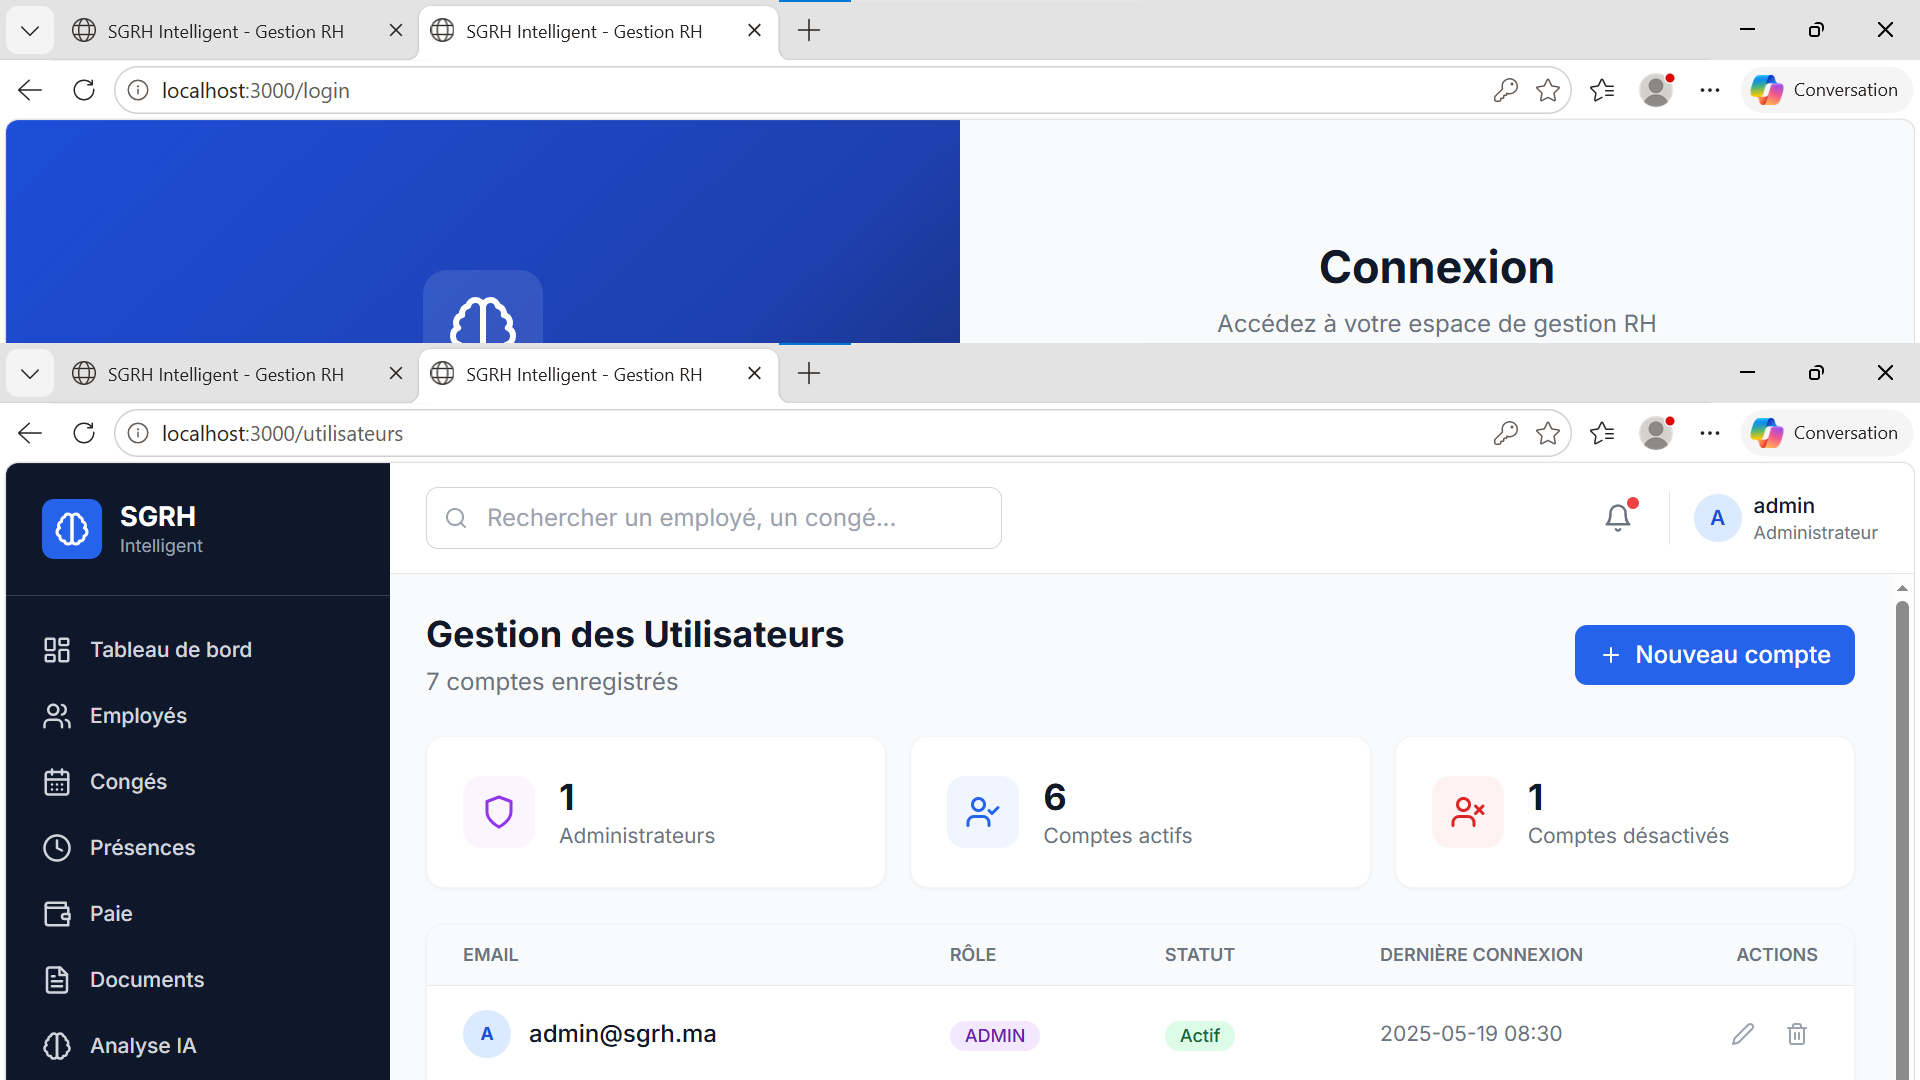
\includegraphics[width=\textwidth]{Gestion_Utilisateurs.png}
\caption{Interface de gestion des comptes utilisateurs}
\label{fig:users}
\end{figure}

\section{Accès}
\begin{itemize}
    \item \textbf{URL} : \texttt{http://localhost:3000/utilisateurs}
    \item \textbf{Fichier source} : \texttt{frontend/src/pages/UsersPage.jsx}
    \item \textbf{Rôles concernés} : ADMIN uniquement
\end{itemize}

\section{Description visuelle}

\subsection{En-tête}

\begin{itemize}
    \item Titre : \og Gestion des Utilisateurs \fg{}
    \item Sous-titre : \og Comptes et droits d'accès \fg{}
    \item Bouton \textbf{+ Nouveau compte} : ouvre un formulaire de création d'utilisateur
\end{itemize}

\subsection{Tableau des utilisateurs}

Le tableau affiche la liste des comptes avec :
\begin{itemize}
    \item \textbf{Email} : adresse email du compte
    \item \textbf{Rôle} : badge coloré — ADMIN (violet), RH (bleu), EMPLOYE (gris)
    \item \textbf{Statut} : badge \og Actif \fg{} (vert) ou \og Inactif \fg{} (rouge)
    \item \textbf{Dernière connexion} : date et heure de la dernière authentification
    \item \textbf{Actions} : icônes modifier (crayon) et supprimer (corbeille)
\end{itemize}

\subsection{Modal de création/modification}

Le formulaire contient :
\begin{itemize}
    \item \textbf{Email} : adresse email du nouveau compte
    \item \textbf{Mot de passe} : mot de passe (hashé en BCrypt côté backend)
    \item \textbf{Rôle} : liste déroulante (ADMIN, RH, EMPLOYE)
\end{itemize}

\section{Comportement fonctionnel}

\begin{itemize}
    \item \textbf{Créer} : POST à \texttt{/api/auth/register} — le mot de passe est automatiquement hashé avec BCrypt
    \item \textbf{Modifier} : permet de changer le rôle ou le statut actif/inactif
    \item \textbf{Supprimer} : confirmation puis suppression du compte
    \item Seul un administrateur peut accéder à cette page (vérification côté frontend et backend)
\end{itemize}

% =============================================================
\chapter{Récapitulatif des interfaces}
% =============================================================

\begin{longtable}{|p{3.5cm}|p{4cm}|p{3cm}|p{3cm}|}
\hline
\textbf{Interface} & \textbf{URL} & \textbf{Rôles} & \textbf{Actions} \\
\hline
Login & \texttt{/login} & Tous & Connexion \\
\hline
Tableau de bord & \texttt{/dashboard} & Tous & Consultation \\
\hline
Employés & \texttt{/employes} & ADMIN, RH & CRUD \\
\hline
Congés & \texttt{/conges} & Tous & Demande, Validation \\
\hline
Présences & \texttt{/presences} & Tous & Consultation \\
\hline
Paie & \texttt{/paie} & ADMIN, RH & Génération, Export \\
\hline
Documents & \texttt{/documents} & Tous & Upload, OCR \\
\hline
Analyse IA & \texttt{/analyse-ia} & ADMIN, RH & Lancer analyse \\
\hline
Utilisateurs & \texttt{/utilisateurs} & ADMIN & CRUD comptes \\
\hline
\end{longtable}

% =============================================================
\chapter{Technologies de l'interface}
% =============================================================

L'interface utilisateur de l'application SGRH Intelligent est construite avec les technologies suivantes :

\begin{longtable}{|p{4cm}|p{9.5cm}|}
\hline
\textbf{Technologie} & \textbf{Rôle} \\
\hline
React 18 & Bibliothèque JavaScript pour la construction d'interfaces utilisateur composées de composants réutilisables \\
\hline
React Router DOM & Système de routage côté client permettant la navigation entre les pages sans rechargement \\
\hline
TailwindCSS & Framework CSS utilitaire permettant de styliser les composants directement dans le code JSX \\
\hline
Recharts & Bibliothèque de graphiques React pour les visualisations (barres, courbes, camemberts, nuages de points) \\
\hline
Axios & Client HTTP pour communiquer avec l'API REST du backend \\
\hline
Lucide React & Bibliothèque d'icônes SVG modernes et légères \\
\hline
React Hot Toast & Système de notifications visuelles (succès, erreur, chargement) \\
\hline
Vite & Serveur de développement rapide et outil de build pour les applications React modernes \\
\hline
\end{longtable}

\section{Principes de design}

L'interface respecte les principes suivants :
\begin{itemize}
    \item \textbf{Responsive} : adaptation automatique aux écrans de bureau, tablette et mobile
    \item \textbf{Cohérence visuelle} : palette de couleurs uniforme, typographie constante, espacement régulier
    \item \textbf{Feedback utilisateur} : notifications toast pour chaque action, animations de chargement, badges de statut colorés
    \item \textbf{Accessibilité} : contrastes suffisants, labels sur les champs, navigation au clavier possible
    \item \textbf{Performance} : chargement rapide grâce à Vite, rendu conditionnel des composants, lazy loading potentiel
\end{itemize}

\end{document}
